% Author: Dr. Matthias Jung, DL9MJ
% Year: 2020
\documentclass[convert = false, border=5pt]{standalone}
\usepackage{fontspec}
\setmainfont{Roboto}
\usepackage[siunitx, straightvoltages]{circuitikzgit}
\usepackage{tikz}


\usepackage{tikz,pgfplots}
\usepgfplotslibrary{fillbetween}
\begin{document} 
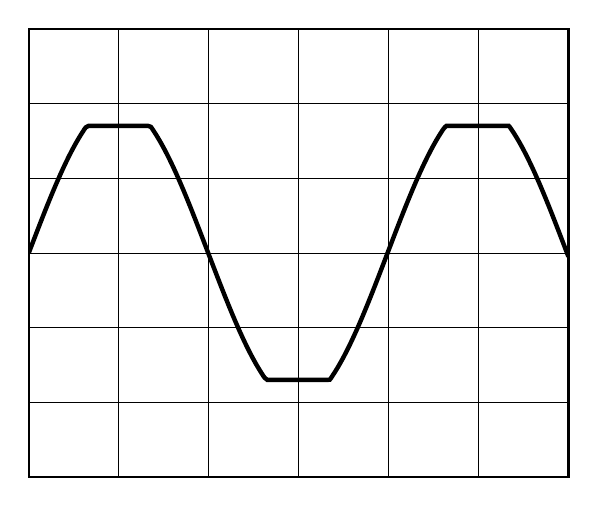
\begin{tikzpicture}
    \pgfplotsset{samples=200}
    \begin{axis}[
        ticks=none,
        xmin =  0,
        ymin = -3,
        xmax =  6,
        ymax =  3,
        domain = 0:6,
        grid=both,
        grid style={line width=.1pt, draw=black},
        major grid style={line width=.2pt,draw=black},
        xtick = {0,1,2,3,4,5,6},
        ytick = {-3,-2,-1,0,1,2,3},
        thick,
        smooth,
        no markers]
    \addplot+[name path=A,ultra thick, black] { max(min(2*sin(deg(x*1.575)-0)+0,1.7),-1.7)};
    \end{axis}
\end{tikzpicture}
\end{document}
